\documentclass{aip-cp}

\usepackage[numbers]{natbib}
\usepackage{rotating}
\usepackage{graphicx}
\usepackage[dvipsnames]{xcolor}

\newif\iffinal
% Un-comment this line to see proposal without comments
%\finaltrue

\iffinal
    \newcommand\ian[1]{}
\else
    \newcommand\ian[1]{{\color{red}[Ian: #1]}}
\fi


% Document starts
\begin{document}

% Title portion
\title{Data Automation at Light Sources:\\Experiments and Lessons Learned\ian{more exciting title needed}}

\author[aff1,aff2]{Author's Name\corref{cor1}}
%\eaddress[url]{address@domain1.edu}
\author[aff2]{Author's Name}
%\eaddress{anotherauthor@thisaddress.yyy}

\affil[aff1]{Data Science and Learning Division, Argonne National Laboratory, Argonne IL 60439, USA.}
\affil[aff2]{Department of Computer Science, University of Chicago, Chicago IL 60637, USA.}
%\affil[aff3]{You would list an author's second affiliation here.}
\corresp[cor1]{Corresponding author: foster@anl.gov}
%\authornote[note1]{This is an example of first authornote.}
%\authornote[note2]{This is an example of second authornote.}

\maketitle


\begin{abstract}
%The AIP Proceedings article template has many predefined paragraph styles for you to use/apply as you write your paper. To format your abstract, use the \LaTeX template style: {\itshape Abstract.} Each paper must include an abstract. Begin the abstract with the word ``Abstract'' followed by a period in bold font, and then continue with a normal 9 point font.
Rapidly growing data volumes at light sources demand increasingly automated data collection, distribution, and analysis processes, in order to enable new scientific discoveries while not overwhelming finite human capabilities. I present here three projects that use cloud-hosted data automation and enrichment services, institutional computing resources, and high- performance computing facilities to provide cost-effective, scalable, and reliable implementations of such processes. In the first, Globus cloud-hosted data automation services are used to implement data capture, distribution, and analysis workflows for Advanced Photon Source and Advanced Light Source beamlines, leveraging institutional storage and computing. In the second, such services are combined with cloud-hosted data indexing and institutional storage to create a collaborative data publication, indexing, and discovery service, the Materials Data Facility (MDF), built to support a host of informatics applications in materials science. The third integrates components of the previous two projects with machine learning capabilities provided by the Deep Learning Hub (DLHub) to enable on-demand access to machine learning models from light source data capture and analysis workflows, and provides simplified interfaces to train new models on data from sources such as MDF on leadership scale computing resources. I draw conclusions about best practices for building next-generation data automation systems for future light sources.
\end{abstract}


% Head 1
\section{INTRODUCTION}

\ian{Potential authors: Ben Blaiszik, Kyle Chard, Ryan Chard, Logan Ward, Justin Wozniak, ...}

TBD.


References: MDF~\cite{MDF2016}, networking materials data~\cite{foster2015networking}, Justin~\cite{wozniak2015big}.


\section{DATA AUTOMATION}

\ian{Big picture thoughts I guess.}

Figures from my 

Choose next experiment.


\section{PRACTICAL EXPERIENCES}

\subsection{Early Work}

We first experimented with online analysis of APS in the late 1990s, 
when we coupled 
computing microtomography~\cite{wang1999quasi,wang2001high} and crystallographic~\cite{von2000using}
experiments to remote computers.
In one memorable demonstration in 1998, we piped microtomography data from APS beamline 2-BM to a 96-node SGI Origin parallel computer 
at Argonne for incremental reconstruction via filtered backprojection as an experiment was proceeding,
and then streamed visualization data to the Supercomputing conference (SC'98) in Orlando, Florida, 
for interactive analysis: see Figure~\ref{fig:sc98}. 
As we noted at the time, 
``the data rates and compute power required ... are prodigious, easily reaching one gigabit per second and a teraflop per second [respectively]"~\cite{von2000using}---numbers that are dwarfed by today's requirements. 

\begin{figure}[h]
  \centerline{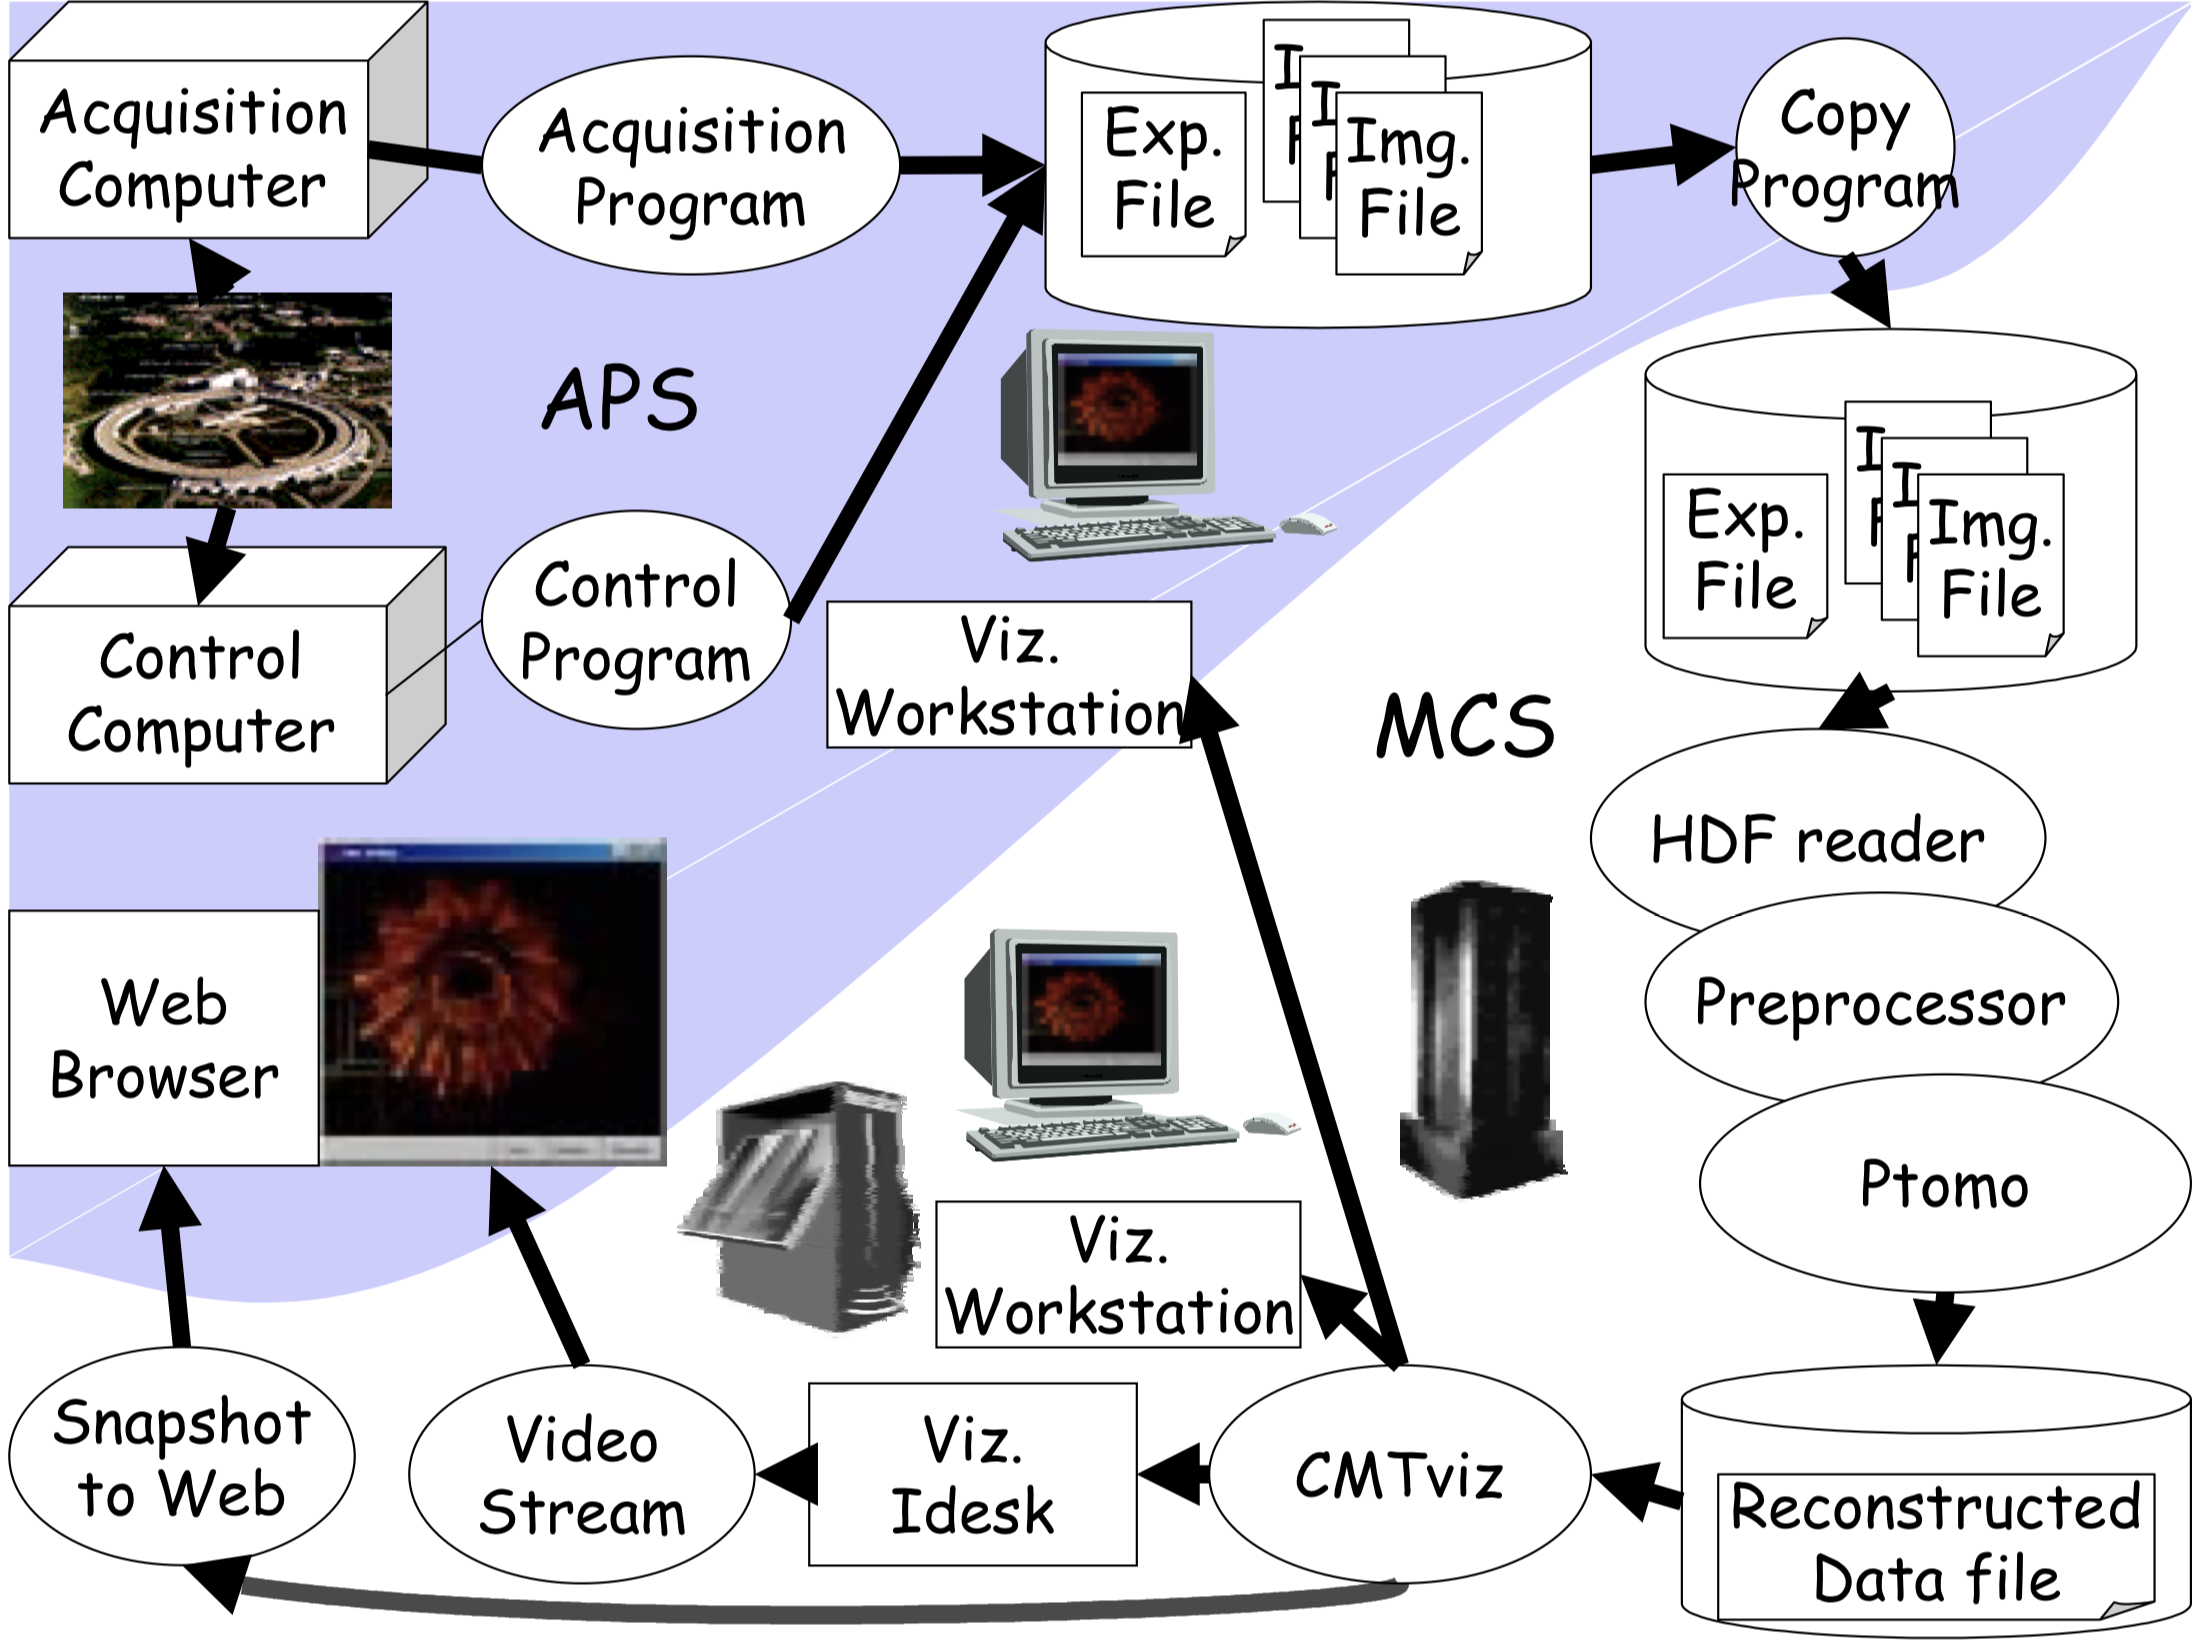
\includegraphics[width=4in]{Figs/APS-Fig.png}}
  \caption{The processing pipeline used in the SC'98 demonstration. Data collected at the APS 
  where passed to supercomputer in Argonne's Mathematics and Computer Science (MCS) division for
  incremental reconstruction and visualization, and results dispatched as a stereoscopic
  video stream to a remote virtual reality displays at APS and in Orlando.\label{fig:sc98}}
\end{figure}

\subsection{Current Status}


\subsubsection{Data acquisition}




\subsubsection{Materials Data Facility}


\subsubsection{DLHub}


\section{RELATED WORK}

Coles et al.~\cite{coles2005ecses,coles2006science} developed an automated small molecule crystallography service that automated the
end-to-end-flow from sample receipt to results dissemination.


\section{SUMMARY}









\section{ACKNOWLEDGMENTS}

This work was supported in part by DOE contract DE-AC02-06CH11357.
We are grateful to colleagues at the Argonne Photon Source and other synchrotron light sources
for many helpful discussions.

% References

\nocite{*}
\bibliographystyle{aipnum-cp}%
\bibliography{Bibs/refs}%


\end{document}
